\subsection{Transistor steuert LED} % (fold)
\label{sub:Transistor_steuert_LED}
\begin{frame}
    \frametitle{Transistor steuert LED}
    \framesubtitle{}
    
\end{frame}
\begin{frame}
    \frametitle{Transistor steuert LED}
    \framesubtitle{Schaltplan}
    \begin{columns}[c]
    \column{.5\textwidth}
        \begin{figure}[H]
        \begin{center}
                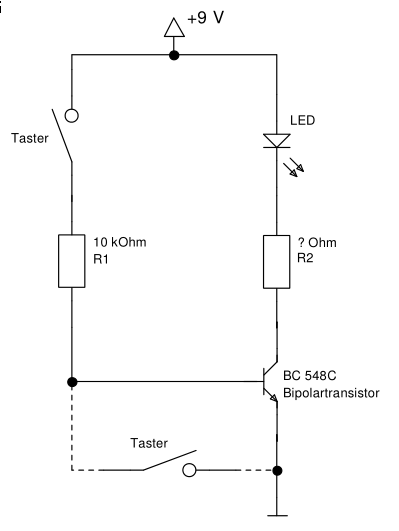
\includegraphics[scale=0.35]{./img/schaltungen/transistorLED_1.png}
        \end{center}
        \end{figure}
    \column{.5\textwidth}
        something something dark side 
    \end{columns}
\end{frame}
\begin{frame}
    \frametitle{Transistor steuert LED}
    \framesubtitle{Schaltplan mit Kurzschluss}
    \begin{columns}[c]
    \column{.5\textwidth}
        \begin{figure}[H]
        \begin{center}
                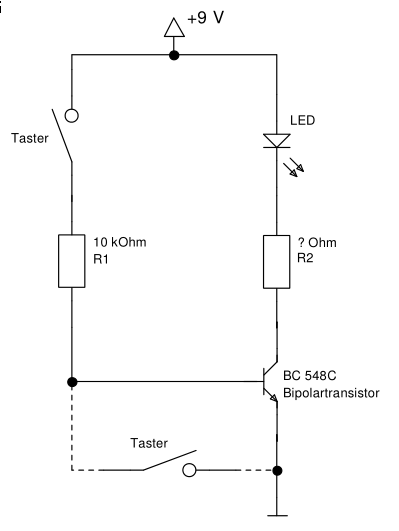
\includegraphics[scale=0.35]{./img/schaltungen/transistorLED_1.png}
        \end{center}
        \end{figure}
    \column{.5\textwidth}
        something something dark side 
    \end{columns}
\end{frame}

% section Transistor steuert LED (end)
